\documentclass[12pt]{article}
\usepackage{graphicx}
\usepackage[margin=1in]{geometry}
\usepackage{setspace}
\usepackage{booktabs}
\usepackage{hyperref}
\usepackage{natbib}

\title{How does Height and Weight Affect NBA Player Performance}

\author{Justin Chan\\
	Jun Yan\\[2ex]
	Department of Statistics\\
	University of Connecticut\\
}

\begin{document}

\maketitle
\doublespace

\begin{abstract}

As basketball players get better and better at their craft in the modern age, players are doing everything 
they can to get an advantage over another. With practice, coaches, and trainers players can work hard at 
mastering their craft but what about the more physical aspects of their game? How does a players' height
and weight impact the performance ability of an NBA Player? Does being taller translate to scoring more
points per game? Does weight increase the amount of rebounds you will grab? Answers to such questions
will offer valuable insight to coaches, scouts, and analysts in making data-driven decisions for their teams.
This paper aims to determine whether, and to what extent, a player's height and weight influence their 
effectiveness in scoring, rebounding, assisting and other metrics through the use of linear regression and
machine learning techniques.

\bigskip
\noindent{\sc Keywords}:
Height and Weight;
Physical;
NBA;
Scoring Ability;
Rebounding Ability;
Assisting Ability;
Linear Regression;
Performance Metrics;
Sports Statistics

\end{abstract}

\section{Introduction}
\label{sec:intro}

Starting with the introduction, the paper will first go into the dataset being used and give a brief summary on the 
variables in the dataset and where the dataset has been collected located in Section~\ref{sec:data}. Following this
will be the Methods section, located in Section~\ref{sec:meth}. This is where the general methodology for the paper
will be explained. The Results section will be next which is where the findings of the research will be found a long 
with any relevant figures. This is located in Section~\ref{sec:resu}. Lastly, the paper will conclude with a Discussion 
section, in Section~\ref{sec:disc} that restates the aim, conclusions, and other important considerations of the paper.
As far as similar research, a study published in the British Journal of Sports Medicine looked at height as a predictor 
within all sports and found that height and sporting success was highly dependent on the type of sport \citep{tucker2012makes}. 
Another study done by head researcher Shaoliang Zhang looked at height and weight as a single predictor along with 
league experience \citep{zhang2017performance}. This paper would build onto that by looking at how player 
performance is affected by height and weight individually within the sport of basketball.

\section{Data}
\label{sec:data}

The dataset used for this analysis is take from Kaggle at \href{https://www.kaggle.com/datasets/justinas/nba-players-data}{NBA Players} 
which sourced its data from the NBA website and Basketball Reference. There are 12.8 thousand observations
with 22 variables taken from 1996 to 2022. It gives the per game averages of each player per season along with
other variables including height and weight. Specifically, the variables include age, games played, points per game,
rebounds per game, assists per game, and net rating. The data has been cleaned with no rows of missing data or
other data quality issues.

Before going into a deeper analysis, it was necessary to prepare the predictor variables to see if they were ready to
be fit within a linear regression model. To check the normality of both the height and weight variables, histograms
were produced:

\begin{figure}
	\caption{Predictor Variable Histograms}
	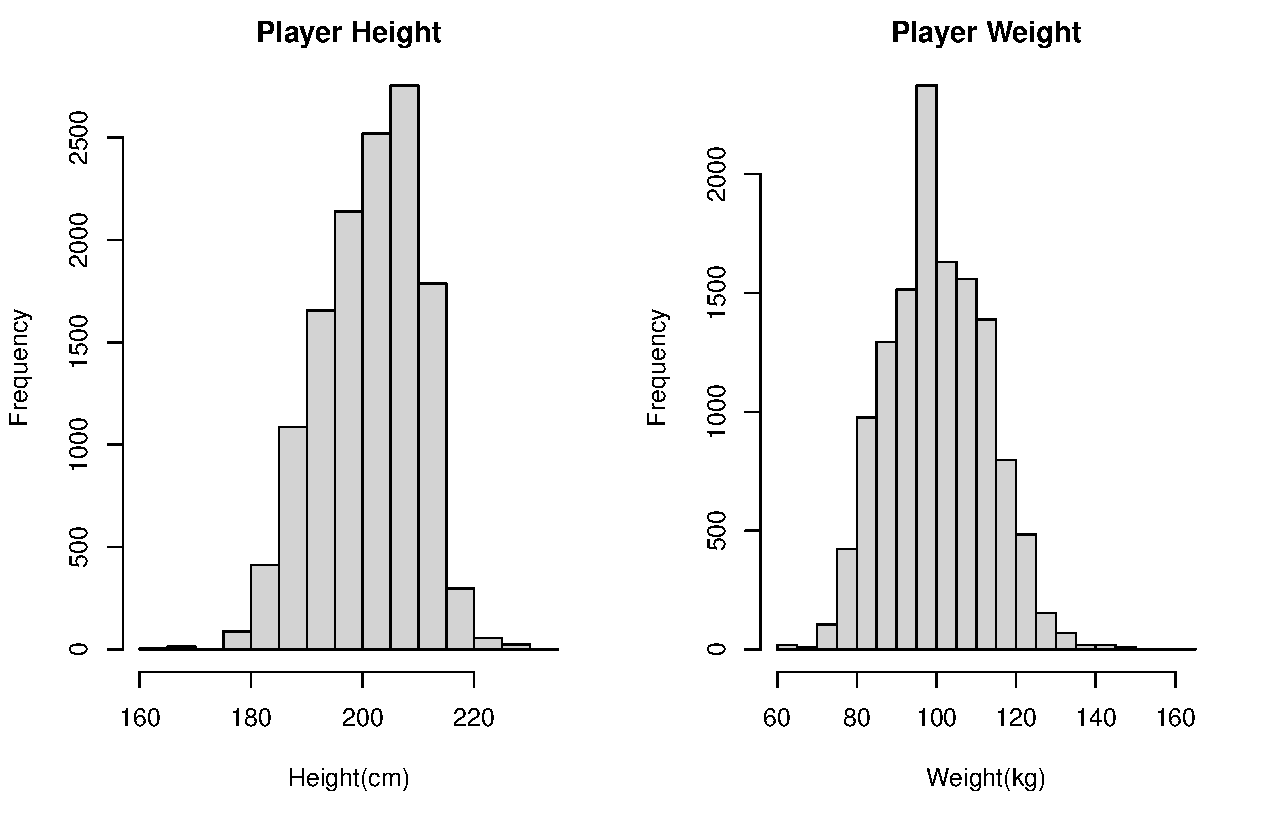
\includegraphics[width=1\textwidth]{predhistograms.pdf}
	\label{fig:predhistograms}
In figure~\ref{fig:predhistograms}, the plots show the distribution of the predictors height and weight.
\end{figure}


\section{Methods}
\label{sec:meth}


\section{Results}
\label{sec:resu}

\section{Discussion}
\label{sec:disc}

\bibliography{references.bib}
\bibliographystyle{plainnat}
\end{document}
	